\documentclass{article}
\usepackage{graphicx} % Required for inserting images
\usepackage{enumerate}
\usepackage{amssymb}
\usepackage[a4paper, total={6in, 8in}]{geometry}
\usepackage{hyperref}
\usepackage{amsmath}
\usepackage{amsthm}
\usepackage{cancel}
\usepackage{tikz} % For drawing shapes


\usepackage{lastpage}
\usepackage{fancyhdr}
\usepackage{geometry}
\geometry{margin=1in}
\usepackage{underscore}
\usepackage{subcaption}
\usepackage{fancyvrb}
\usepackage{listings}
\lstset{basicstyle=\small\ttfamily, columns=flexible, breaklines=true}
\usepackage{tabularx}
\usepackage{float}
\usepackage{makecell}

\usepackage{mdframed}
\usepackage{lipsum}

\usepackage{hyperref}
\usepackage{multicol}
\usepackage{fancyhdr}

\usepackage{xcolor} % For colors
\usepackage{footmisc} % For advanced footnote customization

% Redefine the appearance of footnote markers
\makeatletter
\renewcommand\@makefnmark{%
  \textsuperscript{\textcolor{red}{\fbox{†}}}%
}
\renewcommand\@makefntext[1]{%
  \noindent\textsuperscript{\textcolor{red}{†}} #1%
}
\makeatother


\pagestyle{fancy}
\fancyhf{} % Clear default headers and footers

% Add a simple header
\fancyhead[L]{\textbf{CSE-102 Notes}} % Left-aligned header text
\fancyhead[R]{\textbf{Winter 2025}}   % Right-aligned header text

% Add page numbers in the footer
\fancyfoot[C]{\thepage\ of \pageref{LastPage}} % Center-aligned footer with total pages

% Disable red box around page numbers (using hyperref)
\usepackage{hyperref}
\hypersetup{
    colorlinks=false, % Enable colored links
    linkcolor=blue,  % Set the color of internal links (like page numbers)
    urlcolor=blue,   % Set the color of URLs
    pdfborder={0 0 0} % Remove the border around links
}

\title{CSE-102: Introduction to Analysis of Algorithms\\ Lecture Notes}
\author{Mann Malviya }
\date{Winter 2025}

\begin{document}

\maketitle
\tableofcontents
\newpage

\section*{Introduction}
\addcontentsline{toc}{section}{Introduction} 

\subsection*{Textbooks}
\addcontentsline{toc}{subsection}{Textbooks}

\begin{enumerate}
    \item Algorithms Illuminated, Vols 1,2 and 3 by Tim Roughgarden.
    \begin{figure}[H]
        \centering
        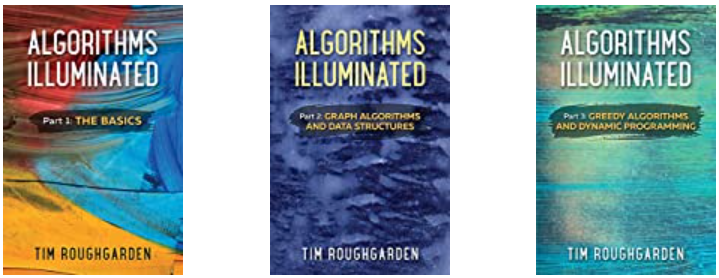
\includegraphics[scale=2]{Algorithms_Illuminated.png}
    \end{figure}

    \item \textbf{"CLRS"} Introduction to Algorithms by Cormen, Leiserson, Rivest and Stein
    \item “Algorithm Design” by Kleinberg and Tardos
    \begin{figure}[H]
        \centering
    \end{figure}

    \begin{figure}[H]
        \centering
        \begin{minipage}{0.48\textwidth}
            \centering
            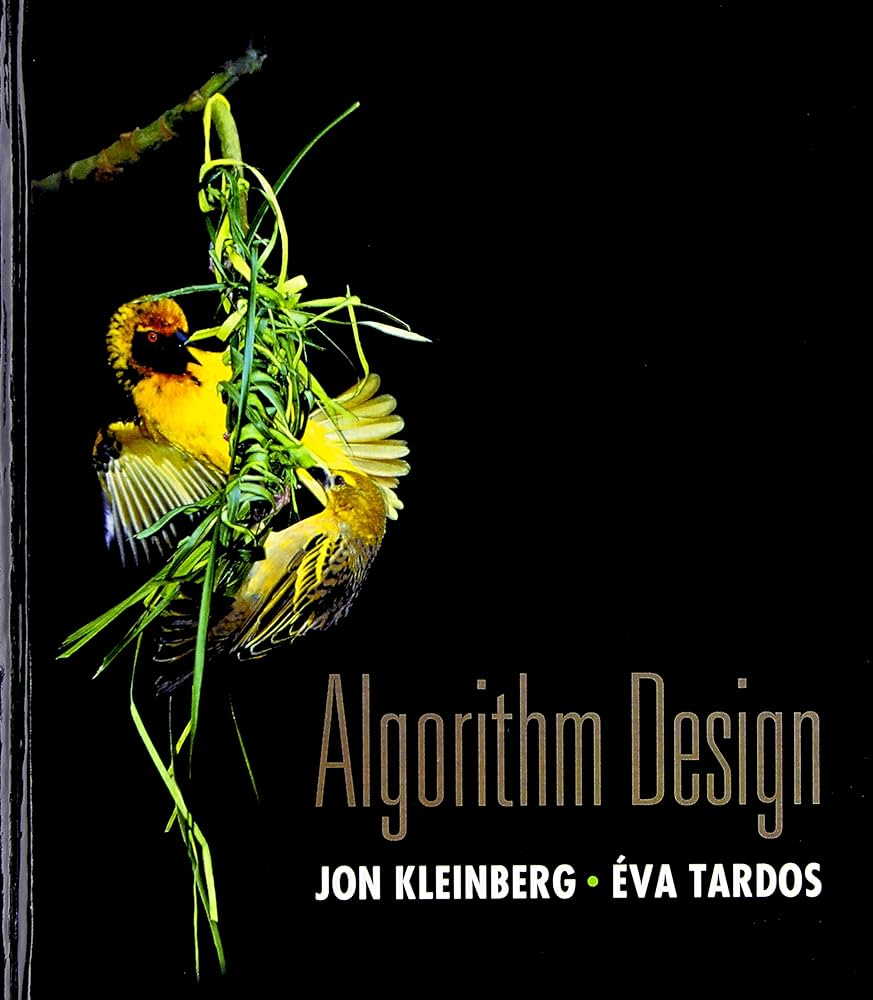
\includegraphics[scale=0.7]{Algorithm_Design.png}
            \caption*{\centering{Algorithm Design by Kleinberg and Tardos}}
        \end{minipage} \hfill
        \begin{minipage}{0.48\textwidth}
            \centering
            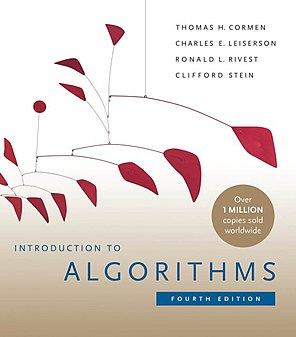
\includegraphics[scale=2]{CLRS.png}
            \caption*{\centering{Introduction to Algorithms \\ by Cormen, Leiserson, Rivest and Stein}}
        \end{minipage}
    \end{figure}

\end{enumerate}
\begin{center}
	\rule{450pt}{1pt} 
\end{center}

\subsection*{What is this Doc?}
\addcontentsline{toc}{subsection}{What is this Doc?}

This doc is my "notes" for the CSE102 course offered at UCSC. I will divide the doc based on each Lecture. For each lecture I shall write down all the important concepts and ideas discussed and their relevant explanations, further I might also add on extra information/elaboration from other sources, thereby making this a comprehensive study resource for me.
\begin{center}
	\rule{450pt}{3pt} 
\end{center}
\newpage

\section*{Lecture 1:}
\addcontentsline{toc}{section}{Lecture 1}

\subsection*{Etymology of "Algorithms"}
\addcontentsline{toc}{subsection}{Etymology of "Algorithms"}

\begin{itemize}
    \item Persian mathematician Muhammad ibn Musa al-Khwarizmi (around 780–850 CE) was a 9th-century scholar, he wrote a book about how to multiply with Arabic numerals.
    \item Al-Khwarizmi $\rightarrow$ Algorismi $\rightarrow$ Algorisme
    \item When his works were translated into Latin in the 12th century, his name was Latinized to Algoritmi.
    \item Originally, “Algorisme” [old French] referred to just the Arabic number system, but eventually it came to mean “Algorithm”.
    \item Al-Khwarizmi's work also gave us the word "algebra", which comes from "al-Jabr," a term used in the title of his book.
\end{itemize}

\subsection*{Integer Multiplication Problem}
\addcontentsline{toc}{subsection}{Integer Multiplication Problem}

\begin{center}
\fbox{%
  \parbox{11cm}{% Adjust 11cm to match the content size
    \centering
    \textbf{Problem: Integer Multiplication}
    \vspace{0.5em}

    \noindent\textbf{Input:} Two $n$-digit nonnegative integers, $x$ and $y$.

    \vspace{0.5em}
    \noindent\textbf{Output:} The product $x \cdot y$.
  }%
}
\end{center}

\

\

The Integer Multiplication Algorithm will transform the Input to the Output.

\begin{itemize}
    \item The way we will assess the performance of this algorithm is through the number of basic(or "primitive") operations that are performed.
    \item "Basic/Primitive/Atomic Operations": Add or Multiply 2 single digit numbers together.
    \item We will count the number of these primitive operations performed by the following multiplication algorithms as a function of the number of digits, $n$.
\end{itemize}

\subsection*{1. Grade-School Multiplication Algorithm}
\addcontentsline{toc}{subsubsection}{Grade-School Multiplication Algorithm}

\[
\begin{array}{r} % Align to the right
  \overbrace{123392570752752384623764...283568364918374523856298}^{\text{$n$}} \\ % The first number with labeled brace
  \times \ \ 562323582342395285623467...235019130750135350013753 \\ % The multiplier with "x"
  \hline % Horizontal line
\end{array}
\]

\begin{itemize}
    \item Assume you are multiplying 2 $n$-digit numbers(if one of the numbers doesn't have $n$-digits you can add leading $0$ to make them so).
    \item Each digit of the bottom number multiplies all the $n$-digits of the top number, hence a total of $n$ single digit multiplication operations are done, further since these multiplications can cause a carry digit, there can be \textbf{at most} $n$ carry digits(even though the first 1-digit multiplication never has carry, don't forget the last digits carry) that need to be added to the product of the single digits
    \begin{itemize}
        \item[$\hookrightarrow$] So the total number of Primitive operations performed for each digit of the bottom number is $n+n = 2n$.
    \end{itemize}
    \item Since the bottom number has $n$ digits, each of those digits will perform $2n$ operations, giving a total of $n\times 2n = 2n^2$ primitive operations performed to obtain all the partial products.
    \begin{figure}[H]
        \centering
        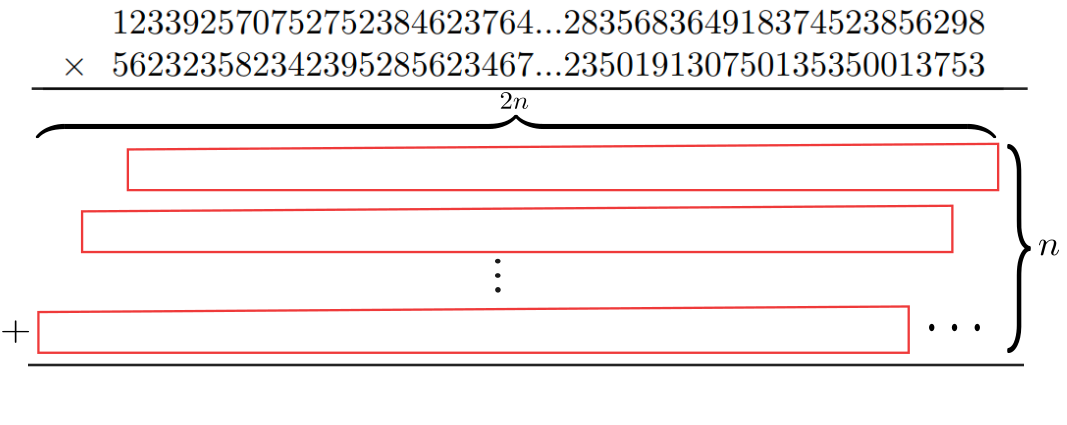
\includegraphics[scale=1.3]{multiplication.png}
    \end{figure}

    \item We still need to add the $n$ partial products produced to get the final answer. So we will count the number of single digit atomic additions that are performed, The number of digits in each partial product must equal the number of digits in the last partial product(this is achieved by padding the other partial products with $0$'s at their start) which is equal to $(n+1)+(n-1)=2n$, each one digit number multiplied by the top number produces $n+1$ digits and $n-1$ zeros must be added at the end as part of the algorithm.
    \begin{itemize}
        \item[$\hookrightarrow$] Each partial product has $2n$ digits and there are $n$ of them, hence a total of $2n\times n=2n^2$ operations will be performed in computing the sum of all the partial products(think of this as adding all the 1-digit numbers in each column, each column has $n$ digits hence $n$ additions must be done and there are $2n$ columns).
    \end{itemize}
    \item So $2n^2$ operations are performed to compute all the partial products and $2n^2$ operations are done in adding them all. A total of $\boxed{4n^2}$ operations are performed to compute the product of two $n$-digit numbers using the grade-school algorithm.
    \item The grade-school algorithm is said to have a time complexity of $n^2$ \footnote{Later Lecture we see the precise time complexity is $\Theta(n^2)$}. By this we are measuring how the runtime scales with the size of the input. We assume each of the atomic operation take the same time.
\end{itemize}


\subsection*{2. Divide and Conquer Algorithms for Multiplication}
\begin{itemize}
    \begin{figure}[H]
        \centering
        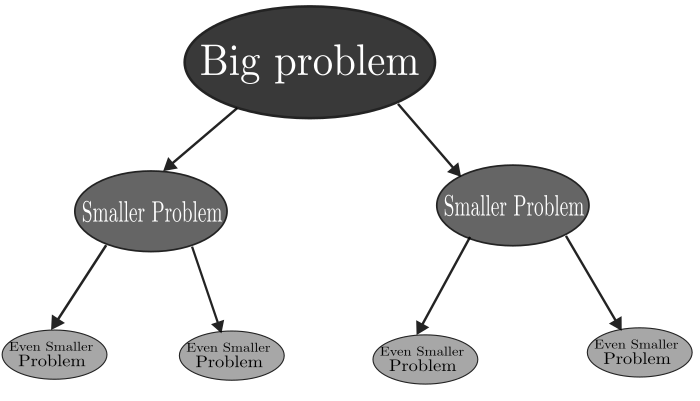
\includegraphics[scale=1.7]{divide_&_conquer.png}
        \centering{\caption*{Divide and Conquer}}
    \end{figure}
    \item We now look for a better algorithm for multiplying two $n$-digit numbers. We shall use the technique of \textbf{Divide and Conquer}.
    \begin{itemize}
        \item[$\hookrightarrow$]The idea being, breaking a big complicated problem into smaller(easier) sub-problems. It is often done \textbf{recursively}.\\ Example: Binary Search, Merge Sort. 
    \end{itemize}
\end{itemize}
\subsection*{2.1 A Recursive Algorithm}
\addcontentsline{toc}{subsubsection}{A Recursive Algorithm}
\begin{itemize}
    \item 
\end{itemize}


\begin{center}
	\rule{450pt}{1pt} 
\end{center}
\newpage

\section*{Lecture 2:}
\addcontentsline{toc}{section}{Lecture 2}

\subsection*{3. Karatsuba integer multiplication}
\addcontentsline{toc}{subsubsection}{Karatsuba integer multiplication}


Formal Defn of Algorithm
Intro of Computational model: RAM model
How to describe algorithms
Proving correctness using Loop invariant and/or PMI
    -> Insertion Sort using LI
    -> Merge Sort using Induction




\begin{center}
	\rule{450pt}{1pt} 
\end{center}
\newpage

\section*{Lecture 3:}
\addcontentsline{toc}{section}{Lecture 3}

Asymptotic notations. Comparing Asymptotic quantities.
Mathematical notations
Use of asymptotic notations in equations



\begin{center}
	\rule{450pt}{1pt} 
\end{center}
\newpage

\section*{Lecture 4:}
\addcontentsline{toc}{section}{Lecture 4}

Recursion tree method

\begin{center}
	\rule{450pt}{1pt} 
\end{center}
\newpage

\section*{Lecture :}
\addcontentsline{toc}{section}{Lecture}

Add the Matrix stuff.\\

\subsection*{Quick Sort}


\end{document}
